\documentclass[a4paper,12pt]{article}

\usepackage{Ai_logo}
\usepackage{graphicx}
\usepackage{amsmath}

\pagestyle{empty}

\begin{document}

\flushleft{\Ai}

\begin{figure}[ht]
    \centering
    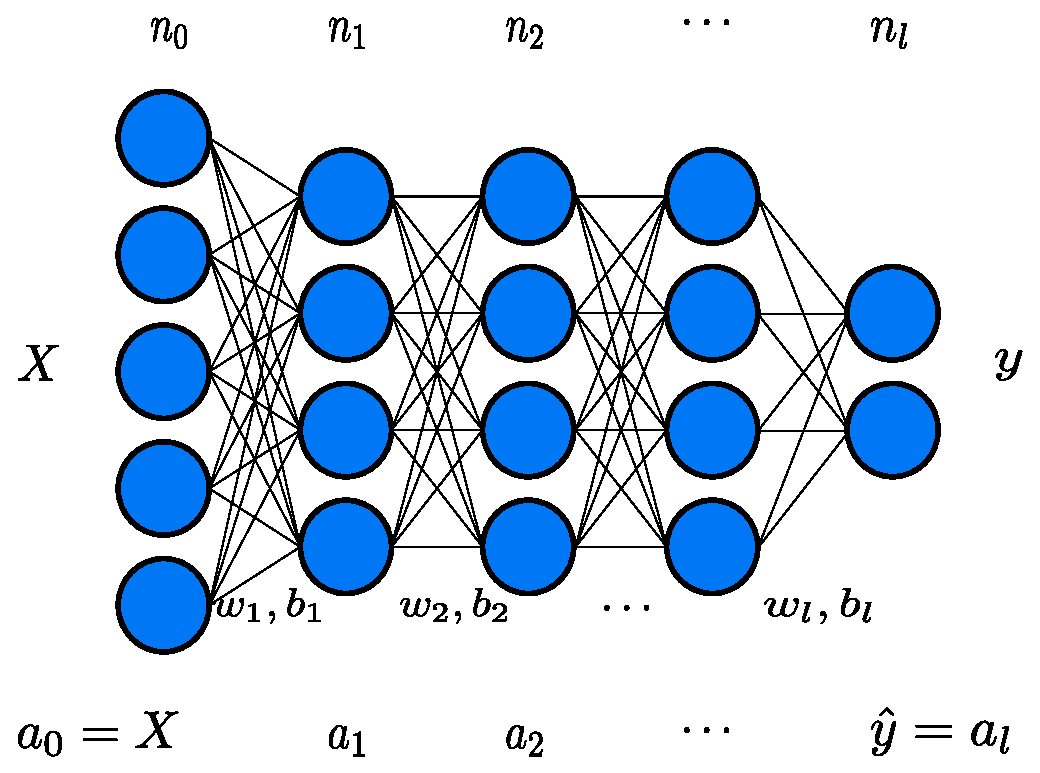
\includegraphics[width = \textwidth]{ann_diagram}
    \caption{ANN diagram}
    \label{fig:ann_diagram}
\end{figure}

\raggedright

Definition:
\begin{displaymath}
    a_i: \ m \Bigg\{
    \underbrace{
    \left( \begin{array}{ccc}
    x_{11} & x_{12} & \ldots \\
    x_{21} & x_{22} & \ldots \\
    \vdots & \vdots & \ddots
    \end{array} \right)
    }_{n_i},
\ 
    w_i: \ n_{i-1} \Bigg\{
    \underbrace{
    \left( \begin{array}{ccc}
    w_{11} & w_{12} & \ldots \\
    w_{21} & w_{22} & \ldots \\
    \vdots & \vdots & \ddots
    \end{array} \right)
    }_{n_i},
\ 
    b_i: \ \underbrace{
    \left[ \begin{array}{ccc} b_1 & b_2 & \ldots \end{array} \right]
    }_{n_i},
\end{displaymath}

\begin{align*}
        a_0 &= X, \\
        a_i &= f_a(a_{i-1}w_i + b_i), \\
    \hat{y} &= a_l, \\
          i &\in [1,l] \textrm{ and } i \in \mathbf{Z^+} .
\end{align*}


activation function: sigmoid($x$)/$\sigma(x)$
\begin{align*}
    f_a(x) = \sigma(x) &= \frac{1}{1 + e^{-x}} \\
             {f_a}'(x) &= \frac{e^{-x}}{(1 + e^{-x})^2} = \sigma(x)(1 - \sigma(x))
\end{align*}


cost function: cross entropy
\begin{equation*}
    C = -\frac{1}{m} \sum_{j = 1}^{m}\sum_{k = 1}^{n_l}[y\ln(\hat{y}) + (1-y)\ln(1-\hat{y})],
    \textrm{ while } \hat{y} = a_l = \sigma(a_{l-1}w_l + b_l)
\end{equation*}

let $z_l = a_{l-1}w_l + b$,
then $a_l = \sigma(z_l)$

when $j \in [1,m], \ k \in [1,n_l], \ k' \in [1,n_{l-1}]$
and $j, \ k, \ k' \in \mathbf{Z^+}$

\begin{flalign*}
    & \textbf{0.1. }
    \frac{\partial C}{\partial a_l^{j,k}}
        = \frac{1}{m} \frac{a_l^{j,k} - y_l^{j,k}}{a_l^{j,k}(1 - a_l^{j,k})}
\\
    & \textbf{0.2. }
    \frac{\partial a_l^{j,k}}{\partial z_l^{j,k}} = a_l^{j,k}(1 - a_l^{j,k})
\\
    & \textbf{0.3.1. }
    \frac{\partial z_l^{j,k}}{\partial a_{l-1}^{j,k'}} = w_l^{k',k}
\\
    & \textbf{0.3.2. }
    \frac{\partial z_l^{j,k}}{\partial w_l^{k',k}} =  a_{l-1}^{j,k'}
\\
    & \textbf{0.3.3. }
    \frac{\partial z_l^{j,k}}{\partial b_l^k} = 1
\\
    & \textbf{1. }
    \frac{\partial C}{\partial a_{l-1}^{j,k'}}
        = \sum_{k = 1}^{n_l}\frac{\partial C}{\partial a_l^{j,k}}
            \cdot \frac{\partial a_l^{j,k}}{\partial z_l^{j,k}}
            \cdot \frac{\partial z_l^{j,k}}{\partial a_{l-1}^{j,k'}}
        = \frac{1}{m} \sum_{k = 1}^{n_l}(a_l^{j,k} - y_l^{j,k})w_l^{k',k}
\\
    & \textbf{2. }
    \frac{\partial C}{\partial w_l^{k',k}}
        = \sum_{j = 1}^{m}\frac{\partial C}{\partial a_l^{j,k}}
            \cdot \frac{\partial a_l^{j,k}}{\partial z_l^{j,k}}
            \cdot \frac{\partial z_l^{j,k}}{\partial w_l^{k',k}}
        = \frac{1}{m} \sum_{j = 1}^{m}(a_l^{j,k} - y_l^{j,k})a_{l-1}^{j,k'}
\\
    & \textbf{3. }
    \frac{\partial C}{\partial b_l^j}
        = \sum_{j = 1}^{m}\frac{\partial C}{\partial a_l^{j,k}}
            \cdot \frac{\partial a_l^{j,k}}{\partial z_l^{j,k}}
            \cdot \frac{\partial z_l^{j,k}}{\partial b_l^k}
        = \frac{1}{m} \sum_{j = 1}^{m}(a_l^{j,k} - y_l^{j,k})
\end{flalign*}

\flushright{\Ai}

\end{document}
